\documentclass[twoside,11pt]{article}

\usepackage{jmlr2e}
\usepackage{booktabs}
\usepackage{multirow}
\graphicspath{{../figures/}}

\newcommand{\benchmark}{\textsc{GeoVLM-Bench}}

\jmlrheading{}{2026}{1-\pageref{LastPage}}{}{}{}{Ashok Sivathayalan and Sai Paladugu}
\usepackage{lastpage}

\ShortHeadings{GeoVLM-Bench}{Sivathayalan and Paladugu}
\firstpageno{1}

\begin{document}

\title{GeoVLM-Bench: A Cue-Structured Benchmark for Evaluating Geographic Visual Reasoning in Vision-Language Models}

\author{\name Ashok Sivathayalan \email ashoksivathayalan@cmail.carleton.ca \\
       \addr School of Computer Science\\
       Carleton University\\
       Ottawa, ON, Canada
       \AND
       \name Sai Paladugu \email saipaladugu@cmail.carleton.ca \\
       \addr School of Computer Science\\
       Carleton University\\
       Ottawa, ON, Canada}

\editor{}

\maketitle

\begin{abstract}
Vision-language models (VLMs) have shown impressive capabilities across a range of multimodal tasks, yet their ability to perform geographic visual reasoning remains poorly understood. Existing geolocation benchmarks report only aggregate accuracy, obscuring which types of visual evidence models can and cannot exploit. We introduce \benchmark{}, a benchmark of 246 street-level images spanning 13 countries and 9 geographic regions, in which every image is annotated with its primary geographic cue type: linguistic (visible text and signage), environmental (vegetation, terrain, climate), or infrastructure (road markings, driving side, vehicle types). We evaluate six VLMs from three providers---Gemini 3 Flash, Gemini 2.5 Flash, Claude Sonnet 4.6, GPT-4o-mini, GPT-5.4-mini, and Claude Haiku 4.5---on country-level geolocation, reporting accuracy broken down by cue type and model. Our cue-structured evaluation reveals systematic differences in how models leverage different categories of geographic evidence, providing more actionable insight than aggregate accuracy alone.
\end{abstract}

\begin{keywords}
  vision-language models, geolocation, benchmark, geographic reasoning, visual cues
\end{keywords}

\section{Introduction}
\label{sec:introduction}

The task of determining where in the world a photograph was taken---geolocation---has long been studied in computer vision \citep{hays2008im2gps}. The game GeoGuessr popularized this challenge, requiring players to identify locations from Google Street View imagery by reasoning about visible cues such as text, vegetation, road infrastructure, and architectural style. Recent work has shown that VLMs can perform this task with varying degrees of success \citep{haas2024pigeon, jay2025precise}, but evaluation has focused on aggregate accuracy metrics, leaving unclear \emph{which types of geographic signals} models can reliably exploit.

This gap matters for several reasons. First, understanding cue-specific strengths and weaknesses informs targeted model improvement. A model that excels at reading signs but fails to interpret vegetation patterns has different failure modes than one exhibiting the opposite behavior. Second, cue-level analysis is relevant to privacy: if models can geolocate images even without readable text---relying instead on subtle environmental or infrastructural cues---this has implications for location privacy in shared imagery \citep{mendes2024gptgeochat}.

Existing geolocation benchmarks for VLMs, including WhereBench \citep{wherebench2025} and GeoRC \citep{talreja2026georc}, evaluate models on geographic reasoning but do not annotate images by the type of geographic cue they contain, making it impossible to attribute model performance to specific reasoning capabilities.

We address this gap with \benchmark{}, a benchmark designed around a cue-structured evaluation framework. Our contributions are:
\begin{enumerate}
    \item A curated dataset of 246 street-level images from Mapillary, spanning 13 countries across 9 geographic regions, where each image is annotated with its primary geographic cue type (linguistic, environmental, or infrastructure).
    \item A subset of 42 multi-cue images annotated with overlapping cue categories, enabling analysis of cue interactions.
    \item A comparative evaluation of six VLMs spanning lightweight to mid-tier from three providers---Google, Anthropic, and OpenAI---with accuracy reported per model, per cue type, and per model-cue combination.
\end{enumerate}

\section{Related Work}
\label{sec:related}

\paragraph{Image geolocation.} Classical approaches to image geolocation frame the problem as image retrieval \citep{hays2008im2gps} or classification over a discretized grid of the Earth's surface \citep{muller2018geolocation}. PlaNet \citep{weyand2016planet} trained a deep CNN to classify images into geographic cells, achieving impressive performance on a large-scale dataset. More recently, PIGEON \citep{haas2024pigeon} combined multi-task contrastive pretraining of CLIP with a GeoGuessr-inspired training regime, achieving superhuman performance on the game. These approaches are task-specific models, whereas our work evaluates general-purpose VLMs.

\paragraph{VLM geolocation benchmarks.} Several benchmarks have recently evaluated VLMs on geolocation. GPTGeoChat \citep{mendes2024gptgeochat} evaluates conversational geolocation with GPT-4V and raises privacy concerns. WhereBench \citep{wherebench2025} provides a multi-scale benchmark from country to precise coordinates. GeoRC \citep{talreja2026georc} evaluates the quality of VLM-generated geolocation reasoning chains against expert-written chains, focusing on explainability rather than prediction accuracy; while GeoRC categorizes the scene attributes experts cite (infrastructure, vegetation, architecture, etc.), it does not pre-annotate images by cue type or use cue categories to structure accuracy evaluation. GEOBench-VLM \citep{danish2025geobench} covers broader geospatial tasks. Jay et al.\ \citep{jay2025precise} benchmark GPT-4o and Claude on street-level geolocation. All of these report aggregate or region-level accuracy, or evaluate reasoning quality orthogonally to cue type; none annotate images by the type of geographic cue they contain to enable the kind of per-cue accuracy analysis we perform.

\paragraph{Geographic cues in geolocation.} The geolocation community has long recognized that different visual cues carry geographic information \citep{hays2008im2gps}. GeoGuessr players develop expertise in reading scripts, identifying vegetation biomes, and recognizing road marking conventions. However, no prior benchmark has systematically annotated images by cue type and used this to structure model evaluation.

\section{The \benchmark{} Benchmark}
\label{sec:benchmark}

\subsection{Design Principles}

\benchmark{} is built around three design goals: (1)~every image should be annotable with a primary cue type, enabling cue-level accuracy breakdowns; (2)~the dataset should span diverse geographic regions to avoid conflating cue-type effects with regional biases; and (3)~evaluation should use country-level accuracy, which is coarse enough to be meaningful for the cue-structured analysis while avoiding the noise of fine-grained coordinate prediction.

\subsection{Image Collection}

Images were sourced from Mapillary, a platform hosting crowd-sourced street-level imagery with open Creative Commons licenses. We selected 13 countries distributed across 9 geographic regions (Table~\ref{tab:dataset}), prioritizing geographic and cultural diversity. For each country, approximately 19 images were collected, yielding a total of 246 images. All images are street-level photographs that contain identifiable geographic cues.

\begin{table}[t]
\caption{Dataset composition by region and country.}
\label{tab:dataset}
\centering
\small
\begin{tabular}{llc}
\toprule
\textbf{Region} & \textbf{Country} & \textbf{Images} \\
\midrule
East Asia & Japan, South Korea & 39 \\
Southeast Asia & Thailand, Indonesia & 39 \\
South Asia & India & 20 \\
Western Europe & Germany, United Kingdom & 38 \\
Northern Europe & Finland & 19 \\
Eastern Europe & Russia & 19 \\
North America & Canada, Mexico & 37 \\
South America & Brazil & 18 \\
Middle East & Turkey & 17 \\
\midrule
\textbf{Total} & \textbf{13 countries} & \textbf{246} \\
\bottomrule
\end{tabular}
\end{table}

\subsection{Cue Type Annotation}

Each image was manually annotated with one of three primary cue types:

\begin{itemize}
    \item \textbf{Linguistic}: The most salient geographic signal in the image is visible text---road signs, shop names, billboards, or other written language that could indicate the country or language of origin. (80 images)
    \item \textbf{Environmental}: The dominant cue is natural---vegetation patterns, terrain type, climate indicators (snow, tropical foliage), or landscape features. (73 images)
    \item \textbf{Infrastructure}: The primary signal comes from built-environment features---road markings, driving side, utility pole styles, vehicle types, or architectural conventions. (93 images)
\end{itemize}

A subset of 42 images was additionally annotated as \emph{multi-cue}, indicating the deliberate presence of more than one cue type (e.g., both visible text and distinctive infrastructure). These images are excluded from per-cue-type accuracy breakdowns and analyzed separately in a multi-cue vs.\ single-cue comparison.

The annotation was performed by the authors, both experienced GeoGuessr players. While this limits scalability, it ensures that the cue type label reflects the annotator's judgment about what a human would rely on to geolocate the image, rather than an automated or proxy signal.

\subsection{Evaluation Protocol}

All models receive the same zero-shot prompt instructing them to (1)~describe geographic cues visible in the image, (2)~reason step by step, and (3)~output a final country prediction in a structured format. The prompt is:

\begin{quote}
\small
\texttt{You are analyzing a street-level image to determine where in the world it was taken.}

\texttt{First, carefully describe the geographic cues you can identify in the image. Consider:}
\begin{itemize}
    \item \texttt{Any visible text, signs, or written language}
    \item \texttt{Vegetation, terrain, and climate indicators}
    \item \texttt{Road markings, infrastructure, and vehicle types}
    \item \texttt{Architectural styles and cultural indicators}
\end{itemize}

\texttt{Then, based on your reasoning, state which country you believe this image was taken in.}

\texttt{Format your response exactly as follows:}\\
\texttt{REASONING: <your step-by-step analysis>}\\
\texttt{COUNTRY: <single country name only>}
\end{quote}

Country predictions are extracted from the \texttt{COUNTRY:} line, normalized to canonical names (e.g., \texttt{UK}~$\rightarrow$~United Kingdom), and compared case-insensitively to the ground truth. Predictions that cannot be parsed are logged as errors.

We additionally compute \emph{region-level accuracy}: whether the predicted country falls within the same geographic region as the ground truth, providing a measure of partial credit for near-miss predictions.

\subsection{Models Evaluated}

We evaluate six VLMs spanning lightweight to mid-tier from three major providers:

\begin{itemize}
    \item \textbf{Gemini 3 Flash} and \textbf{Gemini 2.5 Flash} (Google): fast, cost-efficient models from the Gemini family, accessed via the Google Generative AI API.
    \item \textbf{Claude Sonnet 4.6} and \textbf{Claude Haiku 4.5} (Anthropic): a mid-tier and a lightweight model from the Claude family, accessed via the Anthropic API.
    \item \textbf{GPT-5.4-mini} and \textbf{GPT-4o-mini} (OpenAI): compact variants from OpenAI's recent and previous generation, accessed via the OpenAI API.
\end{itemize}

By evaluating two models per provider, we can observe both cross-provider and within-provider variation. All models receive images as base64-encoded JPEGs with the identical prompt.

\section{Results}
\label{sec:results}

\subsection{Overall Accuracy}

Table~\ref{tab:overall} reports country-level and region-level accuracy for each model across all 246 images. Gemini 3 Flash achieves the highest country-level accuracy at 93.9\%, followed closely by Gemini 2.5 Flash at 92.3\%. Claude Sonnet 4.6 and GPT-4o-mini form a middle cluster (83.3\% and 81.3\%), while GPT-5.4-mini (75.2\%) and Claude Haiku 4.5 (65.4\%) trail behind. Region-level accuracy, which gives partial credit when the predicted country is in the correct geographic region, is notably higher than country-level accuracy for all models (up to 10.2 percentage points for Claude Haiku 4.5), indicating that a substantial fraction of errors are near-misses where the model identifies the correct region but confuses neighboring or culturally similar countries.

\begin{table}[t]
\caption{Overall accuracy by model. Country-level accuracy requires an exact country match; region-level accuracy requires only that the predicted country falls in the correct geographic region.}
\label{tab:overall}
\centering
\begin{tabular}{lcc}
\toprule
\textbf{Model} & \textbf{Country Acc.} & \textbf{Region Acc.} \\
\midrule
Gemini 3 Flash     & 93.9\% & 95.5\% \\
Gemini 2.5 Flash   & 92.3\% & 95.9\% \\
Claude Sonnet 4.6  & 83.3\% & 89.8\% \\
GPT-4o-mini        & 81.3\% & 89.4\% \\
GPT-5.4-mini       & 75.2\% & 85.0\% \\
Claude Haiku 4.5   & 65.4\% & 75.6\% \\
\bottomrule
\end{tabular}
\end{table}

\subsection{Accuracy by Cue Type}

Table~\ref{tab:main} presents the main result: accuracy broken down by model and cue type, computed on the 204 single-cue images (excluding 42 multi-cue images whose primary cue assignment is arbitrary). Figure~\ref{fig:grouped} visualizes these results.

Linguistic cues are the easiest category for all models, with accuracy ranging from 87.0\% (Claude Haiku 4.5) to 100.0\% (Gemini 3 Flash and Claude Sonnet 4.6). Infrastructure cues show the widest spread across models: both Gemini models achieve 98.6\%, while Claude Haiku 4.5 drops to 65.2\%. Environmental cues are the hardest category for every model, with accuracy ranging from 41.5\% to 81.5\%.

\begin{table}[t]
\caption{Country-level accuracy (\%) by model and cue type (single-cue images only). The overall column reports accuracy across all single-cue images for each model.}
\label{tab:main}
\centering
\begin{tabular}{lcccc}
\toprule
\textbf{Model} & \textbf{Linguistic} & \textbf{Environmental} & \textbf{Infrastructure} & \textbf{Overall} \\
\midrule
Gemini 3 Flash     & 100.0 & 81.5 & 98.6 & 93.6 \\
Gemini 2.5 Flash   & 98.6 & 78.5 & 98.6 & 92.1 \\
Claude Sonnet 4.6  & 100.0 & 58.5 & 92.8 & 84.2 \\
GPT-4o-mini        & 95.7 & 61.5 & 79.7 & 79.3 \\
GPT-5.4-mini       & 97.1 & 49.2 & 78.3 & 75.4 \\
Claude Haiku 4.5   & 87.0 & 41.5 & 65.2 & 65.0 \\
\midrule
All models         & 96.4 & 61.8 & 85.5 & 81.6 \\
\bottomrule
\end{tabular}
\end{table}

\begin{figure}[t]
\centering
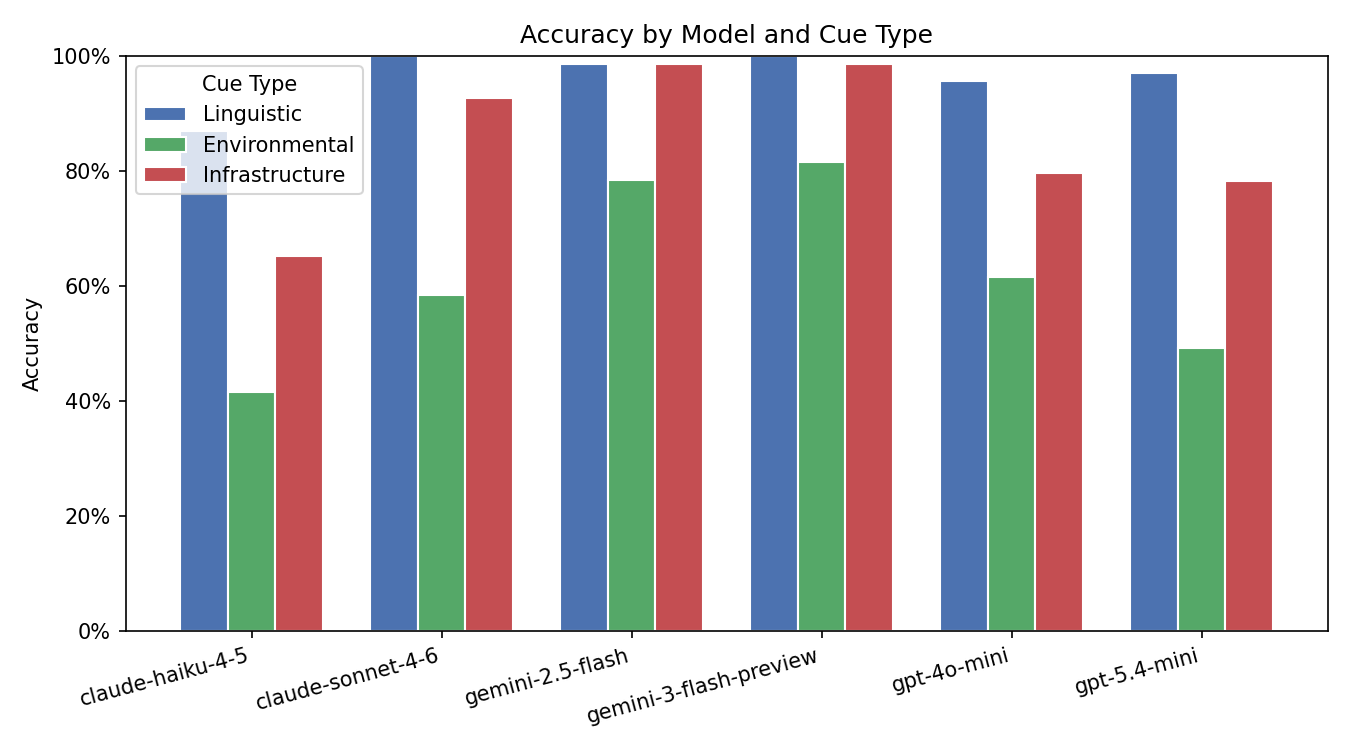
\includegraphics[width=0.85\textwidth]{accuracy_grouped_model_cue.png}
\caption{Country-level accuracy by model and cue type (single-cue images only).}
\label{fig:grouped}
\end{figure}

\subsection{Multi-Cue vs.\ Single-Cue}

Table~\ref{tab:multicue} compares accuracy on single-cue images (204 per model) versus multi-cue images (42 per model). Most models perform better on multi-cue images, with the gap being most pronounced for GPT-4o-mini (+11.4 percentage points). However, two models---Claude Sonnet 4.6 and GPT-5.4-mini---perform slightly worse on multi-cue images, suggesting that redundant cues do not uniformly help and may occasionally introduce conflicting signals.

\begin{table}[t]
\caption{Country-level accuracy (\%) on single-cue vs.\ multi-cue images.}
\label{tab:multicue}
\centering
\begin{tabular}{lcc}
\toprule
\textbf{Model} & \textbf{Single-Cue} & \textbf{Multi-Cue} \\
\midrule
Gemini 3 Flash     & 93.6 & 95.3 \\
Gemini 2.5 Flash   & 92.1 & 93.0 \\
Claude Sonnet 4.6  & 84.2 & 79.1 \\
GPT-4o-mini        & 79.3 & 90.7 \\
GPT-5.4-mini       & 75.4 & 74.4 \\
Claude Haiku 4.5   & 65.0 & 67.4 \\
\bottomrule
\end{tabular}
\end{table}

\section{Discussion}
\label{sec:discussion}

Interpreting linguistic cues appears to be a near-solved problem. All six models achieve at least 87\% accuracy on linguistic images, with Gemini 3 Flash and Claude Sonnet 4.6 reaching 100\%. This is unsurprising: visible text in a distinctive script (e.g., Thai, Japanese, Korean) or language-specific signage provides a strong, unambiguous signal for country identification. The high accuracy here serves as a sanity check that models are meaningfully engaging with the images. Other cue types led to worse performance. Environmental cues (those relying on vegetation and geography) were more difficult for all models, though with high variance of 40 percentage points between the best- and worst-performing models. This is to be expected due to the generic nature of environmental cues - it may often be impossible to differentiate between two tropical regions based only on their vegetation. However, the performance gap suggests that environmental reasoning is still a meaningful indicator of VLM geographic capability. Both Gemini models lead their competitors by nearly 20 points, achieving 81.5\% and 78.5\%, while the remaining four models cluster between 41.5\% and 61.5\%.

Infrastructure cues (road markings, driving side, vehicle types) occupy a middle ground in difficulty. Both Gemini models handle them nearly as well as linguistic cues (98.6\%), while Claude Haiku 4.5 drops to 65.2\%. The 33.4 percentage point spread suggests that infrastructure reasoning---recognizing road conventions, utility pole styles, and vehicle makes as geographically informative---varies substantially across model families. This ordering follows general intuition about cue difficulty: linguistic cues are often unambiguous, infrastructural cues can be region- or country-specific but require more specialized knowledge, and environmental cues are inherently difficult to interpret.

Region-level accuracy is substantially higher than country-level accuracy for all models (Table~\ref{tab:overall}), with gaps ranging from 1.6 percentage points (Gemini 3 Flash) to 10.2 percentage points (Claude Haiku 4.5). This indicates that a significant fraction of country-level errors are near-misses where the model correctly identifies the geographic region but confuses countries within it. The effect is largest for the weaker models, suggesting that regional reasoning develops before precise country discrimination.

Most models perform better on multi-cue images (Table~\ref{tab:multicue}), with the effect strongest for GPT-4o-mini (+11.4 percentage points), suggesting that redundant cue types provide additional signal. However, Claude Sonnet 4.6 and GPT-5.4-mini perform slightly worse on multi-cue images, indicating that the benefit of redundant cues is not universal and may depend on how a model integrates competing signals. With only 42 multi-cue images per model, these differences may not be statistically significant.

Upgrading to a newer model within the same provider family did not uniformly improve performance. While Claude Sonnet 4.6 and Gemini 3 Flash outperformed their lightweight counterparts, Claude Haiku 4.5 and Gemini 2.5 Flash respectively, GPT-5.4-mini performed worse than GPT-4o-mini. This indicates that geographic reasoning does not necessarily improve with newer or more capable models, highlighting the value of a benchmark specifically designed to measure it.

\section{Conclusion}
\label{sec:conclusion}

We presented \benchmark{}, a cue-structured benchmark for evaluating geographic visual reasoning in VLMs. By annotating each image with its primary geographic cue type---linguistic, environmental, or infrastructure---our benchmark enables a more granular analysis of model capabilities than aggregate accuracy alone. Our evaluation of six VLMs from three providers reveals that linguistic cues are near-solved, infrastructure cues discriminate between models, and environmental cues remain substantially challenging for all models tested. These results demonstrate the value of cue-structured evaluation and suggest that improving environmental and infrastructure reasoning should be a priority for VLM geographic capabilities.

\paragraph{Limitations.} Our benchmark has several limitations. The dataset contains 246 images across 13 countries, which is sufficient for cue-level analysis but limits statistical power for fine-grained country-level comparisons. Cue type annotation is inherently subjective; both annotators are experienced GeoGuessr players, which may bias cue classifications toward signals that trained players find salient (e.g., distinguishing infrastructure subtleties like bollard styles or road surface types) rather than cues a naive observer would prioritize. Country-level accuracy, while appropriate for our analysis, does not capture the full spectrum of geolocation precision. Finally, while we evaluate six models spanning lightweight to mid-tier, frontier-tier models may exhibit different performance in response to cues.

\paragraph{Future work.} Natural extensions include scaling the dataset to more countries and images, evaluating frontier-tier models (e.g., Claude Opus, GPT-4o, Gemini Pro), and investigating whether chain-of-thought prompting or cue-specific prompting can improve performance on weaker cue types. A finer-grained cue taxonomy---distinguishing, for example, between Latin-script and non-Latin-script linguistic cues---could yield additional insight.

\acks{This work was completed as a course project for COMP 4900A (Generative AI and Large Language Models) at Carleton University, Winter 2026.}

\bibliography{references}

\end{document}
